\chapter{MOS Capacitor}
The MOS in MOS capacitor stands for Metal-Oxide-Silicon. Sometimes the S is also written as substrate in other places. Understanding threshold voltage here for a MOS-CAP is useful for also understanding MOSFETs in a later chapter.
\begin{pline}
    \item Metal: usually this ia  heavily doped polysilicon (Poly-$Si$) layer doped with $n^+$ or $p^+$, due to high temperature processing for aluminum
    \item Oxide: SiO$_2$ where $\epsilon_{ox} = 3.9 \epsilon_0$, can be any insulator actually
    \item Substrate: $\epsilon_s = 11.7 \epsilon_0$; NMOS capacitor $\rightarrow$ $P$-type substrate, PMOS capacitor $\rightarrow$ $N$-type substrate
\end{pline}

\section{MOSCAP at Equilibrium}
\begin{figure}[H]
    \centering
    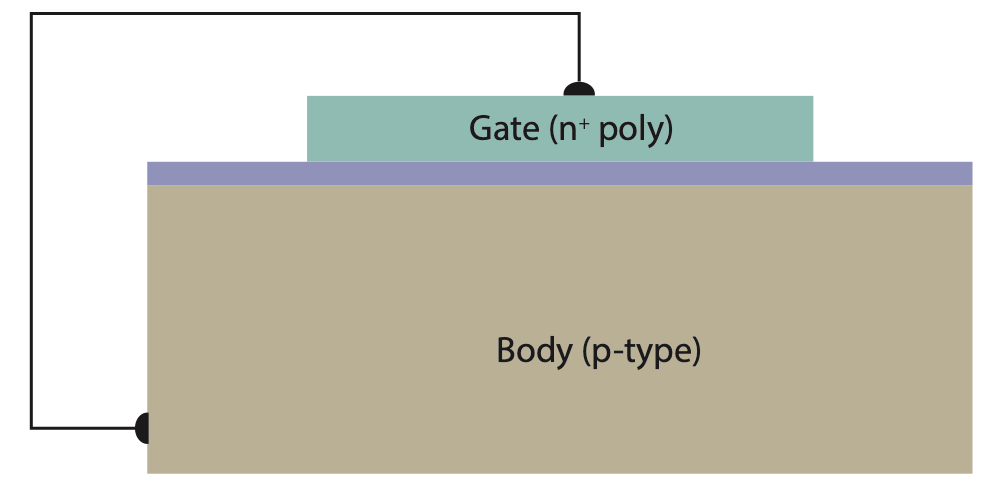
\includegraphics[scale=0.4]{figs/ch04/moscap_short.png}
    \caption{MOS CAP with gate and body shorted in equilibrium}
    \label{fig:moscap_short}
\end{figure}
In equilibrium , the gate and body, which are the terminals where voltage is applied, are shorted like in fig \ref{fig:moscap_short}. Under thermal equilibrium, there is no current flow, so an $N$ type polysilicon gate will rise to a higher potential than the $P$ type substrate like in a PN junction (previous chapter is relevant here). We also assume that the material used to short the body and the gate is made of the gate material, so it looks more like this.
\begin{figure}[H]
    \centering
    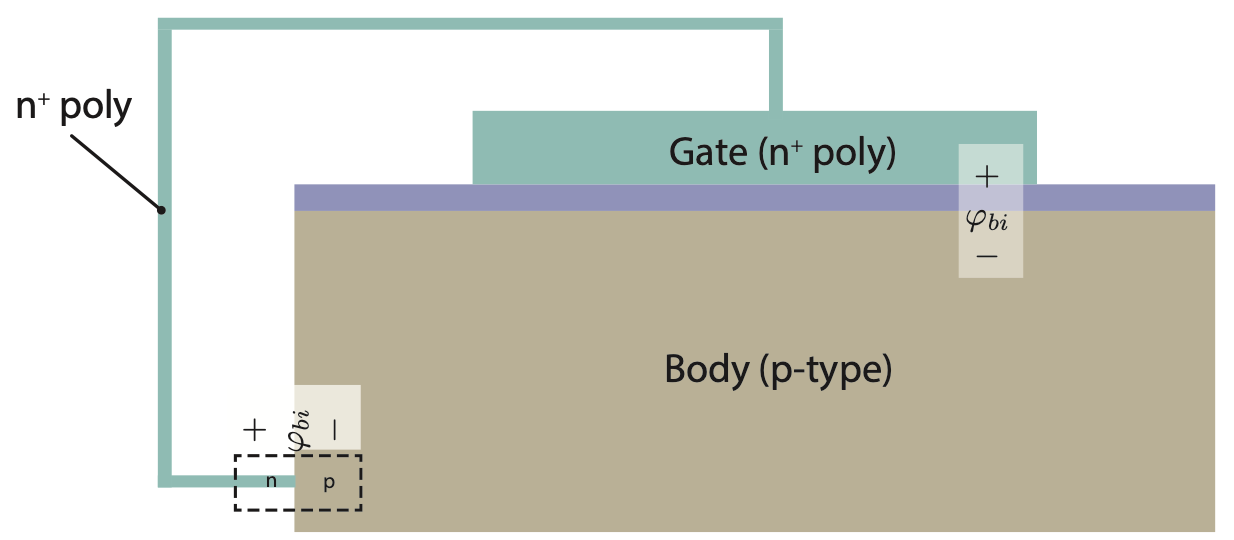
\includegraphics[scale=0.4]{figs/ch04/moscap_short2.png}
    \caption{There is a $\phi_{bi}$ from across the PN junction that leads to potential drop across the oxide}
\end{figure}

\begin{gline}
    \item[] Potential of the $P$ type region substrate: $\phi_p = -(\frac{kT}{q}) \ln(\frac{N_A}{n_i})$ 
    \item[] Potential of the $N$ type gate: $\phi_{poly,n+} = (\frac{kT}{q}) \ln(\frac{N_{d,poly}}{n_i})$
    \item[] Built in potential, NMOS Cap: $\phi_{bi} = \phi_{poly,n+} - \phi_p$
\end{gline}
In practice, real wires made of metal like aluminum or copper are used to connect the gate to the body. At the body side, this metal is connected to a heavily doped $p^+$ region. The \textbf{flatband voltage}, $V_{FB}$, is defined as the gate to body voltage that results in net zero charge and zero fields in the MOSCAP structure. The name comes from the observation that energy bands are flat whe the charge on the gate goes to zero and the depletion region disappears.
    \[V_{FB} = -\phi_{bi} = -(\phi_{n^+} - \phi_p)\]

Due to the difference in materials that make up the gate and body, we have an electric field from the gate to the body. 
\section{Regions of Operation}
There are three regions of operation: accumulation, depletion, and inversion. 

\subsection{Accumulation}
The MOSCAP operates under accumulation when $V_{GB} < V_{FB}$. $V_{GB}$ is the gate to body voltage. This looks like a parallel plate capacitor where there are many electrons and holes to charge up the plates. Negative charges/electrons can flow into the gate and holes will \textbf{accumulate} on the surface of the device. This is because negative bias attracts holes to reside under the gate. 

\subsection{Depletion}
The MOSCAP operates under depletion when $V_{GB} > V_{FB}$. An artificial depletion region is formed if you apply a voltage to the gate of the MOS CAP. When this happens we are in depletion mode. This is similar to the MOS CAP being in equilibrium.

\subsection{Inversion}
The MOSCAP operates under inversion when $V_{GB} = V_{FB}$.
\begin{todo}
    \item might be a good idea to expand on this
\end{todo}

\section{Practice Problems}

\section{Sources}
\begin{itemize}
    \item 
\end{itemize}